%******************************************************************************%
%                                                                              %
%                  ft_boardgame.en.tex for LaTeX                               %
%                  Made by : Michael Lu (mlu@student.42.fr)                    %
%                                                                              %
%******************************************************************************%

\documentclass{42-en}


%******************************************************************************%
%                                                                              %
%                                    Header                                    %
%                                                                              %
%******************************************************************************%
\begin{document}



                           \title{ft\_boardgame}
                          \subtitle{Reinforcing Object Oriented Programming}
                       \member{Michael Lu}{mlu@student.42.fr}
\summary {
  This project is about creating a boardgame utilizing basic Object Oriented
  Programming concepts and class interactions
}

\maketitle

\tableofcontents


%******************************************************************************%
%                                                                              %
%                                  Foreword                                    %
%                                                                              %
%******************************************************************************%
\chapter{Foreword}

	Have you ever wondered what to do if your game fails?\\

	More interesting information about video games. We'll be using Ragnarok Online,
	one of the most popular 2.5d MMORPG. Yes, this is the same development team
	Gravity that had some of the core member move to IMC to make Tree of Saviors
	(if you read the foreword in the previous project). Why would we use Ragnarok
	Online as an example for a failed game if the game was so successful?

	\begin{center}
		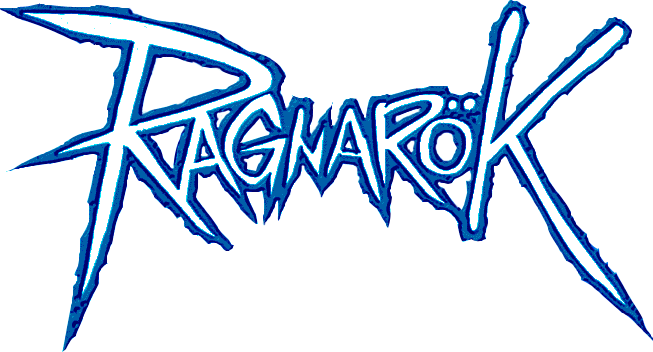
\includegraphics[width=0.6\textwidth]{images/ragnarok.png}
	\end{center}

	Main reason is how they wanted to extend the legacy of Ragnarok Online by making
	a sequel MMORPG, called Ragnarok Online 2. Shortened for RO2 it was a very
	difficult game compared to RO1 (Ragnarok Online, the successful one) since it went
	from a 2.5d MMORPG to a full fledge 3d MMORPG.\\

	First, because the game was so successful the level of hype was incredible. Everyone 
	was expecting a MMO to blow every other competitor out of the water. Second, it still
	had the same core team as the previous RO1 so people were hoping for what made
	RO1 special to be present in RO2. Lastly, the third point is they had promised
	alot of unique mechanics that no other MMORPG had implemented. This was all RO1
	MMORPG players dreamt of. A successful sequel that held the charm of the first game
	and introduced new mechanics that no other game could match.\\

	As you could guess they did succeed in implementing these new mechanics they promised. 
	A combat system no other MMORPG ever made, a unique world and leveling progession.
	Weapon and armor system was completely new, including how quest and rewards were
	handed out. So if this was the case, why did it fail so hard? The overly ambitious
	developers wanted to work so hard on creating a new experience they forgot the most important
	factor of Ragnarok Online 2: Gates of the New World (RO2's full name), and that
	it was NOTHING like Ragnarok Online 1. This left many fans dissapointed in the world,
	the game and everything about it. The backlash was so harsh that they had to make drastic changes.
	This including scrapping the ENTIRE GAME, replacing MOST of the developers and creating
	a new Ragnarok Online 2 called Legend of the Second.\\

	Needless to say, RO2: Legend of the Second is still alive today but it's just a generic
	MMORPG clone that focused more on bringing in the Ragnarok Online 1 theme. The game
	is no where as successful as RO1 and most of the developer went to work on Tree of Saviors
	which is also no where as successful as RO1. In this case, the developers replaced their
	team and even remade the game to try and appease fans. It's quite a difficult 
	time for Ragnarok Online fans like myself because the odds of these talented developers
	ever making a true Ragnarok MMORPG sequel may never happen because of their first time experience.\\

	Hopefully you learned a bit more about MMORPG games and how people have handled it.
	There are more information about this out there, but being a Ragnarok Online 1 fan, I followed
	everything on the RO2 development very closely. Needless to say the only thing that
	could fill that empty fanboy void is Tree of Savior, or playing Ragnarok Online 1 again.
	Sadly, RO2 is not worth it and does not live up to anyone's expectation. (I personally enjoyed
	the first Ragnarok Online 2: Gates of the New World MUCH MORE than the remade version).\\

	\hint {
		Another interesting fact, if you want to see another example of what happens when a game
	fails but succeeded in fixing it, check out the history behind Final Fantasy 14 MMORPG.
	}

%******************************************************************************%
%                                                                              %
%                                 Introduction                                 %
%                                                                              %
%******************************************************************************%
\chapter{Introduction}

	The goal of this project is to create a boardgame with some simple mechanics
	for you and your friends to play. One of the main thing you will be doing is
	continuing to improve on your object oriented skills, and working on reinforcing
	those concepts as well as learning about new concepts to help you make this
	project even better. We will explore a bit more about entities/containers,
	modules and extending clas methods which Python and Ruby both utilizes
	in their object oriented programming.\\


	\warn{
		If you are using python or another language approved by hack high school
		 make sure to research into python equivalent
		concepts on your own. This project can be completed in any
		 approve project language,
		however the tutorial and video guides will be in Ruby.
	}

	So let's talk about how to make a boardgame. First, you need to create the
	spaces/tiles on the boardgame. Second, you need to setup how you will display
	your board. Third, you need to work on a win condition. Afterwards, you will
	have to setup the players and any unique mechanics. In this project, you will
	be making cards/event cards for players to utilize as they progress around the
	board trying to win. Won't be as easy as the previous project, but you can do it!\\



%******************************************************************************%
%                                                                              %
%                                  Goals                                       %
%                                                                              %
%******************************************************************************%
\chapter{Goals}

	The goal of ft\_aboardgame is to help you reinforce your object oriented programming.
	By the end of this project you should know how to:\\
	
	\begin{itemize}
		\item Extend class method
		\item Utilize containers/entities
		\item Utilize modules
		\item Create multiple interactions between objects and classes
		\item Be awesome\\
	\end{itemize}
	 
	You will be exploring a fundamental topic of object oriented programming
	so take advantage of all the resources including the video, your neighbor
	and google. There are many tutorials on classes and inheritance.


%******************************************************************************%
%                                                                              %
%                             General instructions                             %
%                                                                              %
%******************************************************************************%
\chapter{General instructions}

	    \begin{itemize}
		\item This project will only be corrected by actual human beings.
		You are therefore free to organize and name your files as you wish,
		although you must respect some requirements listed below
		\item Your must have a parent class and a children class (they do not
		need to be named parent/children, but it should be easy to see
		which is the children and which is the parent)
		\item A container/entity class is required for your project
		
		\hint{
			It will help you alot to practice writing your entity/container
			first since they help you store multiple instances of object/classes.
			Create a container, store your classes inside and practice creating
			the behaviors inside.
		}	
				
		
		\item Your project must be written in a language approved by
		the hack high school program
		\item All children classes must be unique from one another
		\item You must have a menu/selection screen with proper loop handling
		\item You must allow the ability for people to create a player for the boardgame
		\item You can decide what variables you need for your boardgame
		\item You must display your boardgame in a GUI
		\item Your game must support at least two players
		\item Ask your peers, mentor, slack or anywhere else if you need
		any help, and make sure to have fun\\
	\end{itemize}



%******************************************************************************%
%                                                                              %
%                             Mandatory part                                   %
%                                                                              %
%******************************************************************************%
\chapter{Mandatory part}

		\warn{
			The image example on this PDF are only examples, not what you need
			to replicate. You can design your output, your menu, etc. however
			you would like to design it. If you need help with design please
			visit the tutorial video guides as there is a demo there for you to
			see how the project should behave
		}

	\begin{itemize}

		\item The goal of this project is to create a simple boardgame project
		\item At the beginning of the program the users should be able
		to create a character or see a menu to do so
		\item Containers is required to hold your multiple classes
		\item Container must be able to store your objects/classes, delete them as well as access them
		\item Your boardgame should be made up of tiles/spaces that are children classes
		of a parent class. Your tiles/spaces should be anything from doing nothing,
		to giving players some kind of event or item (ex. move forward X amount of space,
		or give a player a card where they can steal points)
		\item The players must be given an option to roll their dice, or play their
		item/card that they earned from the boardgame
		\item You can choose to end the game immediately after someone wins, or have
		players keep playing
		\item You must display the boardgame in some sort of GUI. This means
		you can decide on what graphic library you want to use for this. Below is
		an example of a simple terminal GUI output

		\begin{center}
			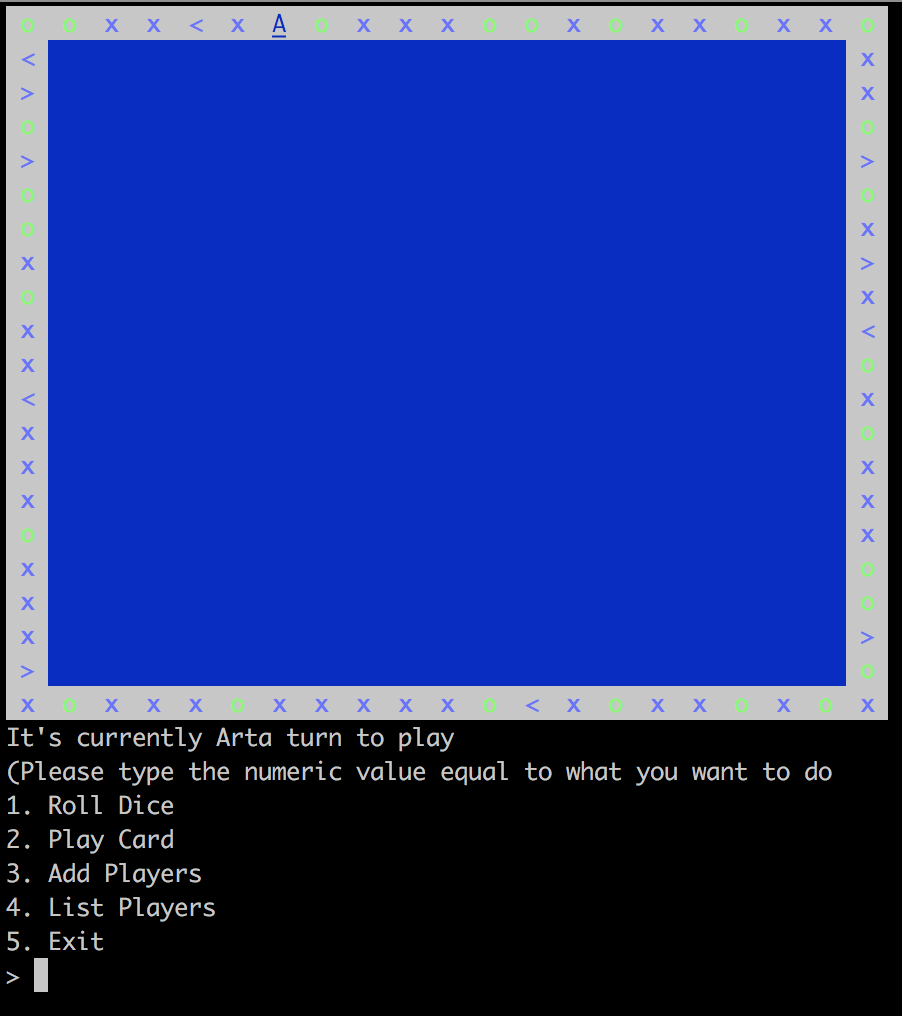
\includegraphics[width=0.6\textwidth]{images/boardgame.png}
		\end{center}

		\item You can design the player class freely as you'd like
		\item You must have the player class equip/hold/contain the items/cards/etc. that
		they can earn through the game
		\item When a player uses an item/card/etc. you must delete that item/card/etc. instance from 
		your player or container
		\item To really emphasize class interaction you will be required to do the following:

		\begin{itemize}
			\item A minimum of three items/cards/etc. that players can earn from playing
			\item All cards/items/etc. are unique children classes that inherits from the same parent class
			\item A minimum of three unique tiles/spaces that does some sort of event
			\item All tiles/spaces are unique children classes that inherits from the same parent class
			\item A container that holds all instances of your classes
		\end{itemize}

		\hint{
			Below is a sketch of what you should considering trying out if you are stuck and unsure
			of how to implement your classes in your container. You do not need to follow this outline,
			this is just here as a guide.
		}

		\begin{center}
			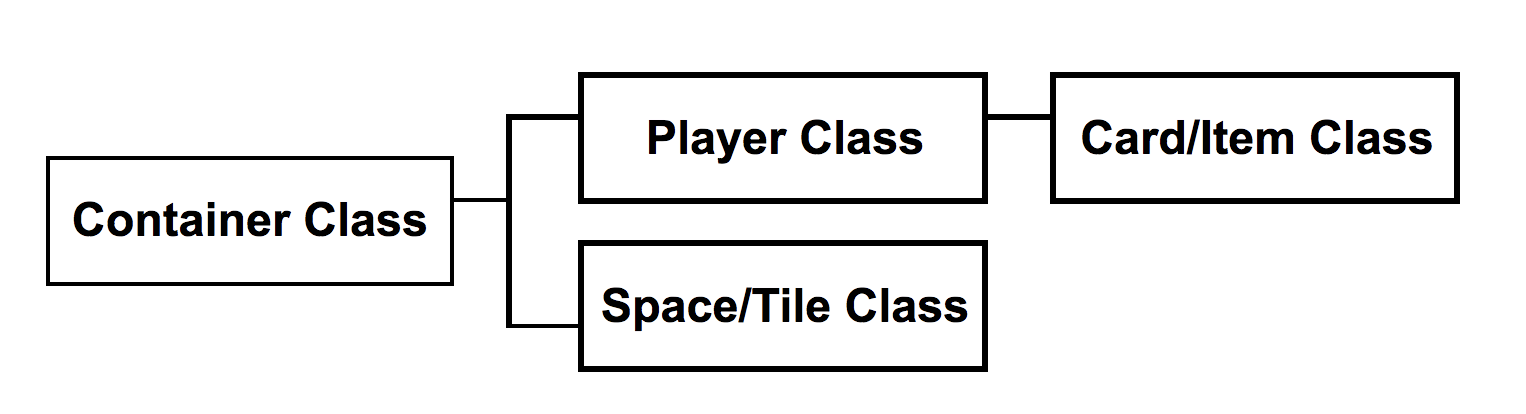
\includegraphics[width=0.6\textwidth]{images/container.png}
		\end{center}

		\item You should try to make the user experience as enjoyable as
		possible. For this reason the GUI should be easy to understand
		\item You must handle any kind of user error to the best of your
		ability. 
		
	\end{itemize}

%******************************************************************************%
%                                                                              %
%                                 Bonus part                                   %
%                                                                              %
%******************************************************************************%
\chapter{Bonus part}
	
	This is a boardgame so you have many opportunities to earn bonus points.
	Make this games yours, be creative and come up with any crazy ideas you have!
	Below are bonuses suggestions, you can do any bonus you think is cool too!
	However, one part of the bonus will be reserved for use of modules and
	class method extensions

	\begin{itemize}
		\item Sound effects
		\item More event/items
		\item Cool effects on the GUI
		\item Additional mechanics, or randomness to the game
		\item Any other cool features you can come up with to enhance
		your boardgame!
	\end{itemize}



%******************************************************************************%
%                                                                              %
%                           Turn-in and peer-evaluation                        %
%                                                                              %
%******************************************************************************%
\chapter{Turn-in and peer-evaluation}

    Turn your work in using your \texttt{GiT} repository, as
    usual. Only work present on your repository will be graded in defense.\\

	Good luck and remember to have fun!



%******************************************************************************%
\end{document}
